
Additional plots and tables.
Hyperparameter settings.
Extended implementation details.




\subsection{ROOT reading and tensorization logic}

\begin{landscape}
    \begin{figure*}
    %\centering
    \hspace{-3cm}
    \vspace{-0.7cm}
    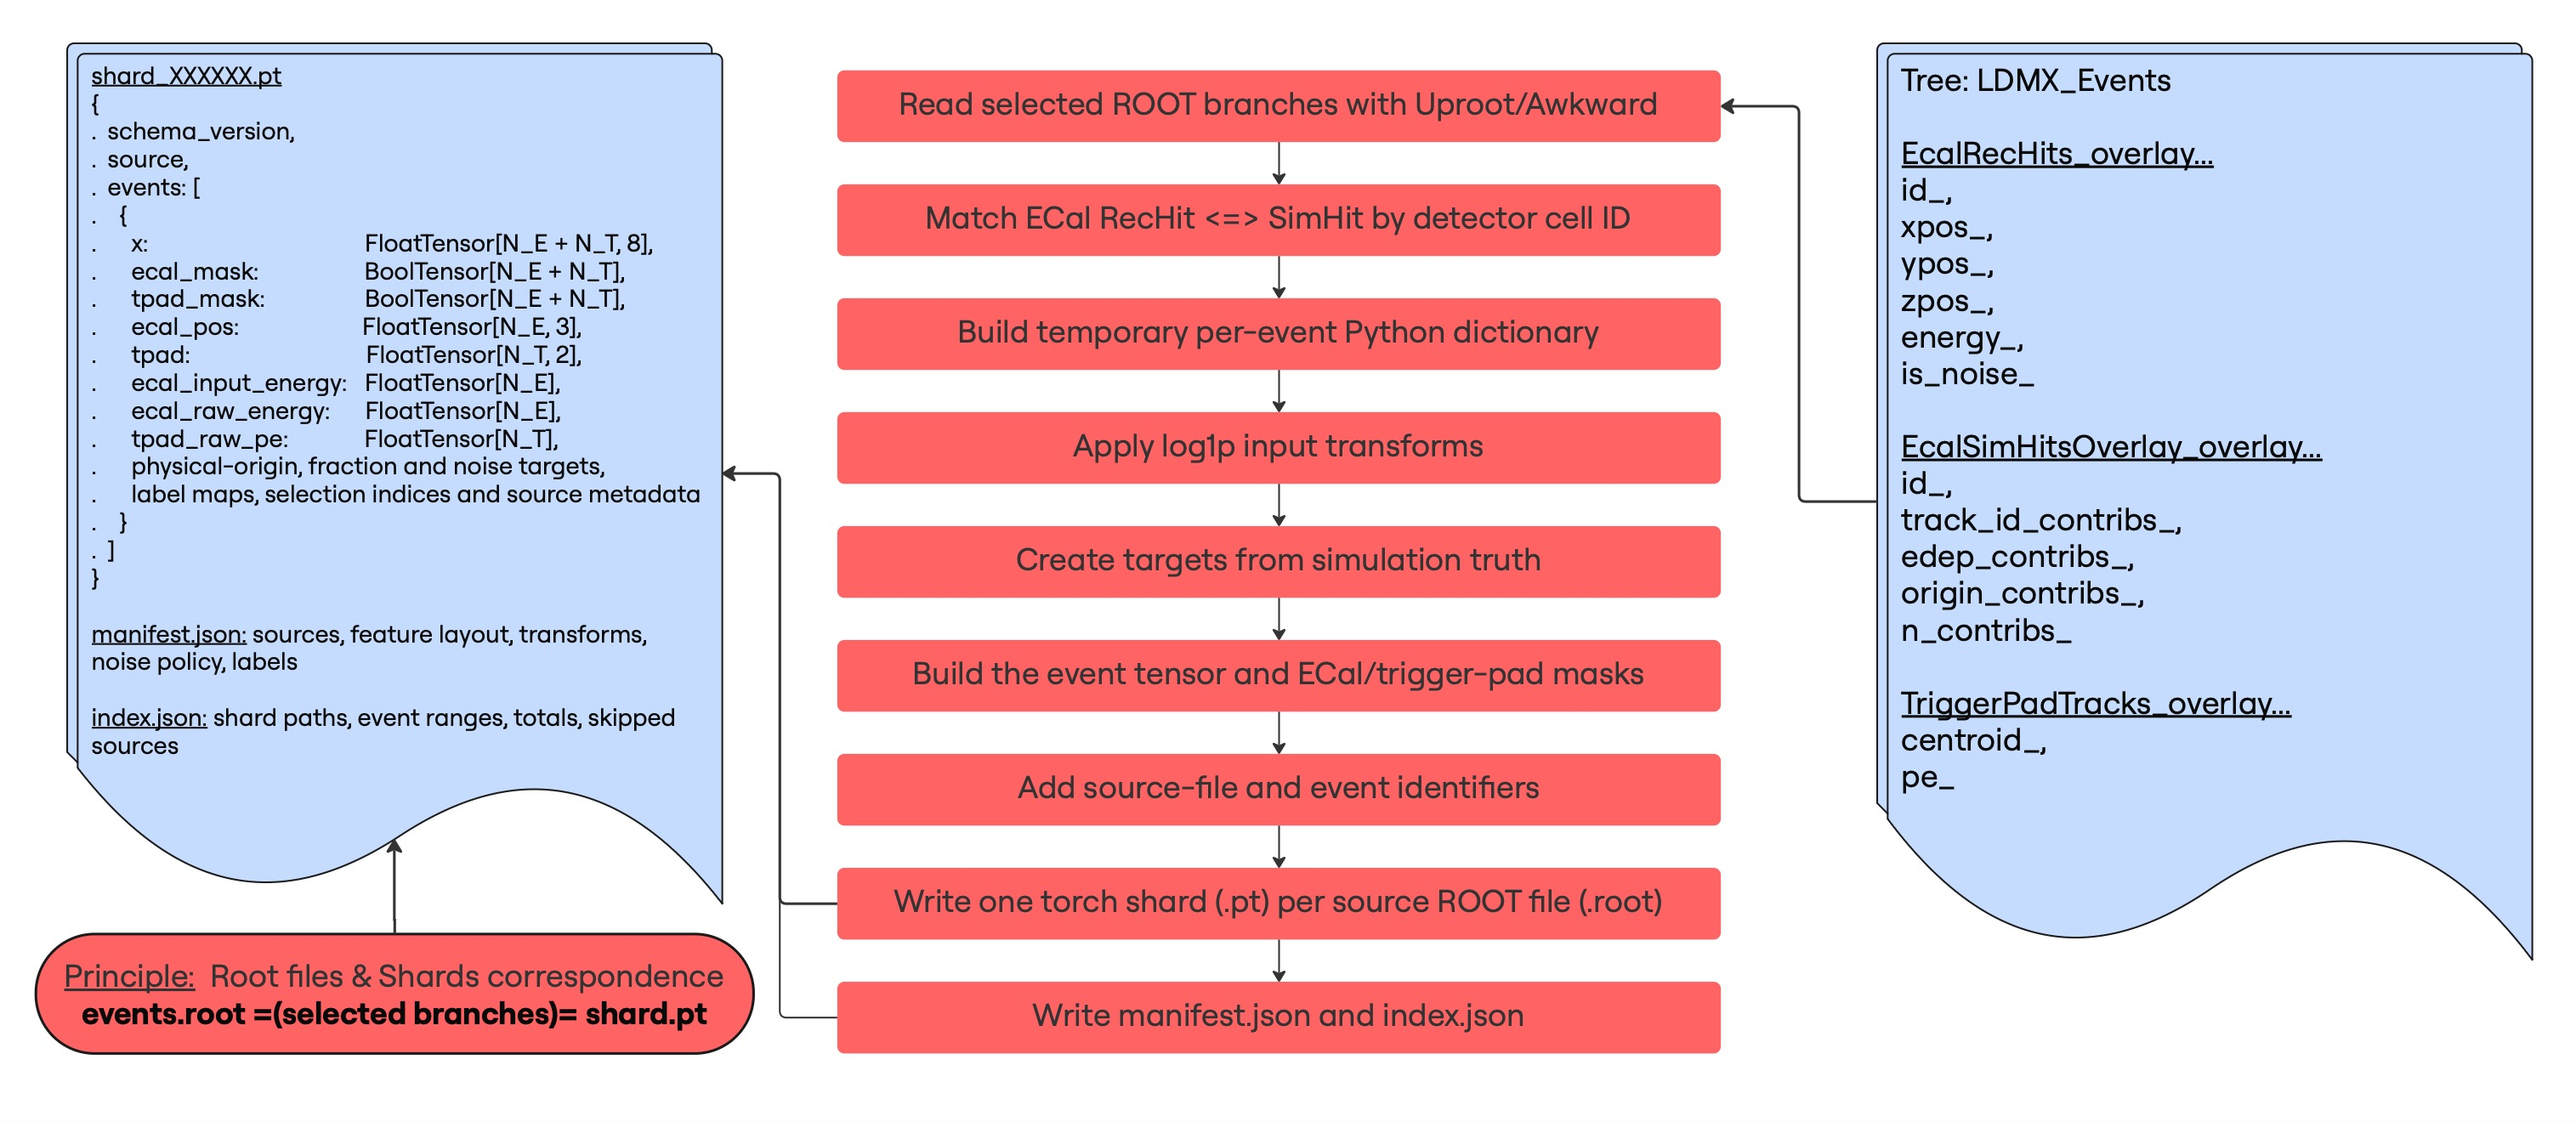
\includegraphics[height=12cm]{config/fig/io_and_tensor.jpg}
    \vspace{-0.5cm}
    \caption{Write caption here...}
    \label{fig:io_and_tensor}
    \end{figure*}
\end{landscape}\makebox[0pt]{}



\subsection{Interactive 3D \gls{ecal} Event Display}

\begin{figure}[H]
    \centering
    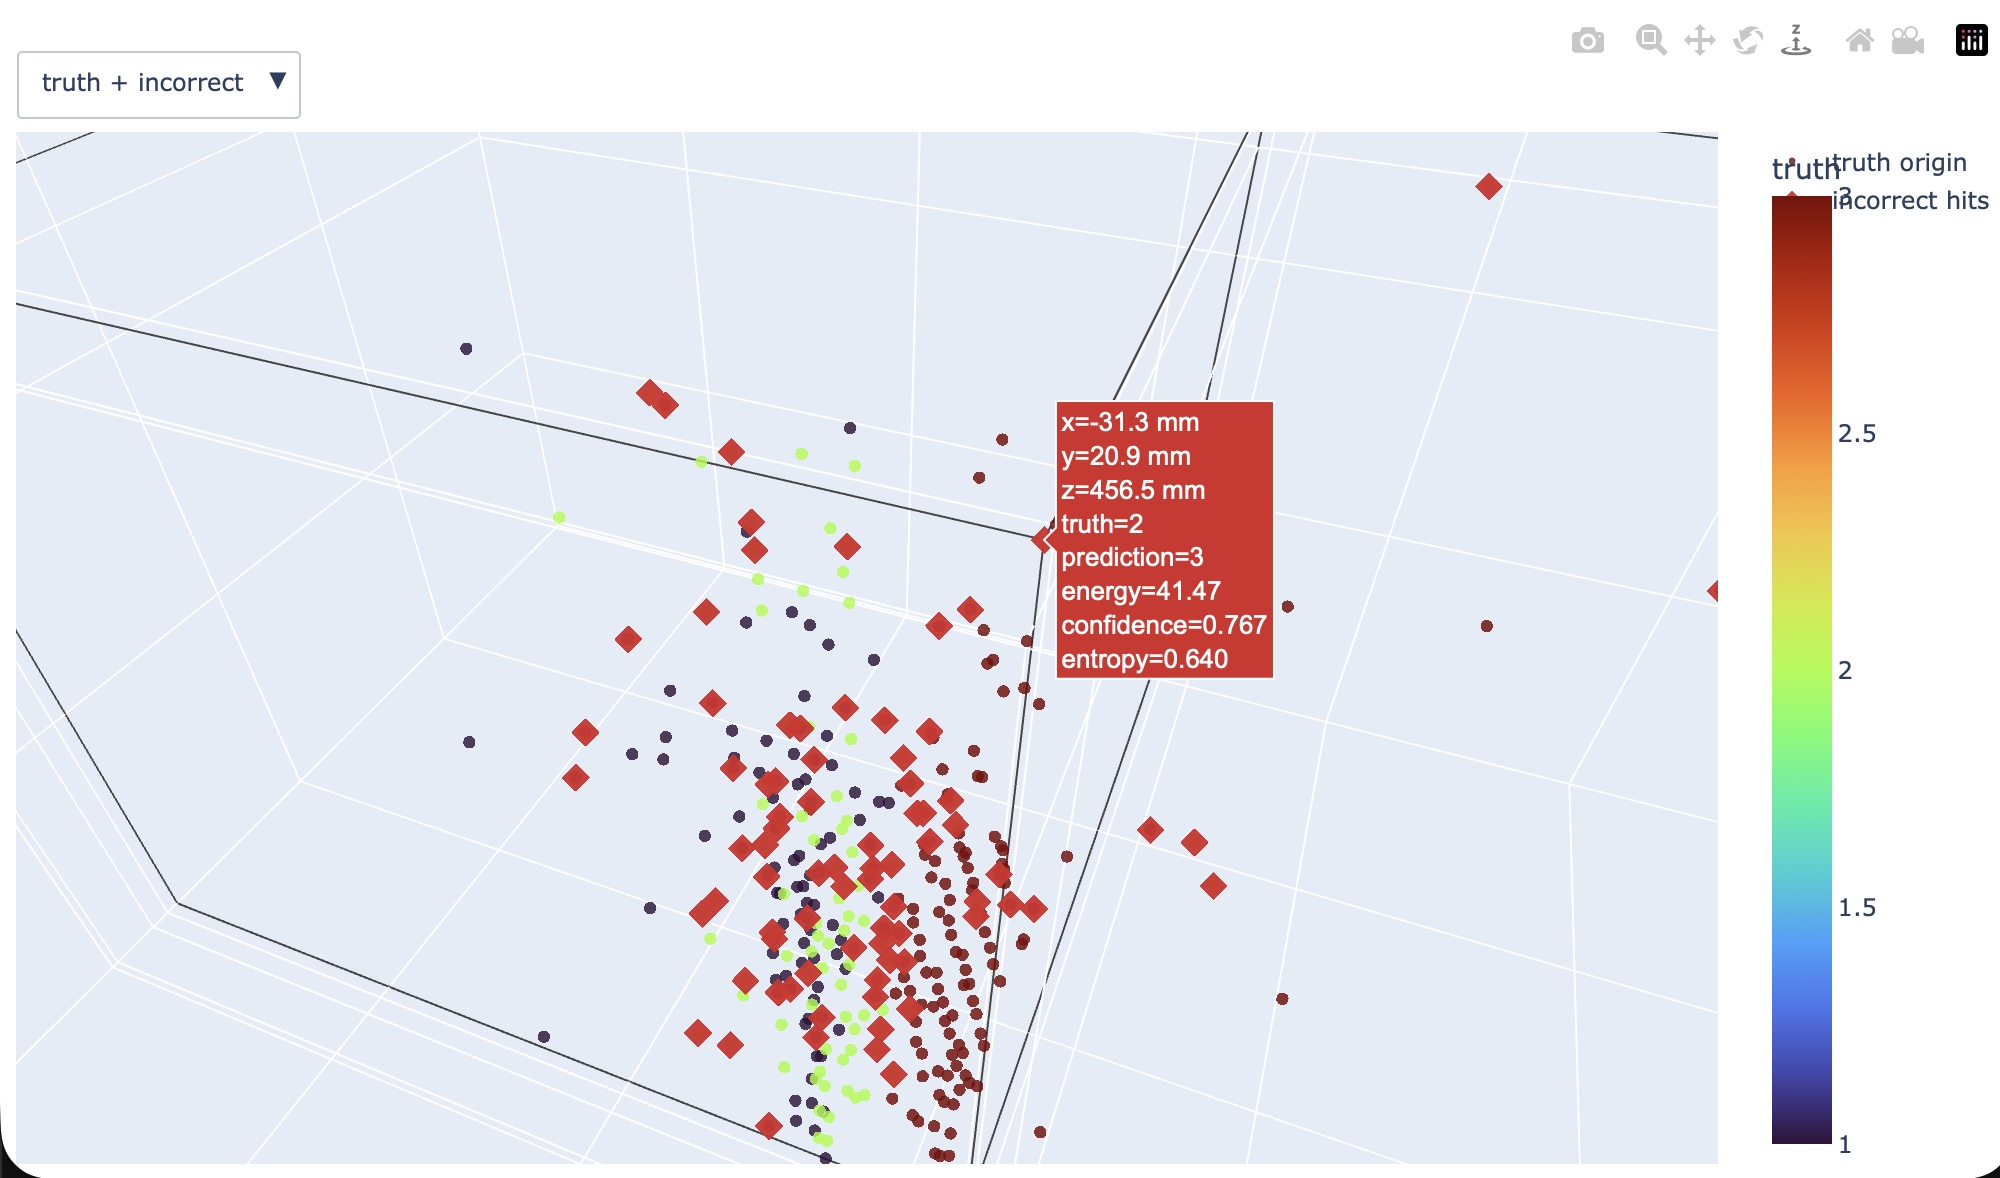
\includegraphics[width=1\linewidth]{config/fig/interactive_event_display.jpeg}
    \caption{Screenshot of the 3D interactive \gls{ecal} event display of a 3e event opened in a browser. The truth + incorrect view is selected in the drop down menu and correctly predicted hits have their respective true label coloring and incorrect predictions are marked in red squares. The user hovers the mouse over an incorrectly predicted \gls{ecal} hit that displays more information about it.}
    \label{fig:interactive_event_display}
\end{figure}


